\documentclass{article} % Especially this!

\usepackage[english]{babel}
\usepackage[utf8]{inputenc}
\usepackage[margin=1.5in]{geometry}
\usepackage{amsmath}
\usepackage{amsthm}
\usepackage{amsfonts}
\usepackage{amssymb}
\usepackage[usenames,dvipsnames]{xcolor}
\usepackage{graphicx}
\usepackage[siunitx]{circuitikz}
\usepackage{tikz}
\usepackage[colorinlistoftodos, color=orange!50]{todonotes}
\usepackage{hyperref}
\usepackage[numbers, square]{natbib}
\usepackage{fancybox}
\usepackage{epsfig}
\usepackage{soul}
\usepackage[framemethod=tikz]{mdframed}
\usepackage[shortlabels]{enumitem}
\usepackage[version=4]{mhchem}
\usepackage{listings}
\usepackage{epstopdf}


\epstopdfDeclareGraphicsRule{.gif}{png}{.png}{convert gif:#1 png:\OutputFile}
\AppendGraphicsExtensions{.gif}
%%%%%%%%%%%%%%%%%%%%%%%%%%%%%%%%%%%%%%%%%%%%%%%%%%%%%
\setlength{\marginparwidth}{3.4cm}


% NEW COUNTERS
\newcounter{points}
\setcounter{points}{100}
\newcounter{spelling}
\newcounter{english}
\newcounter{units}
\newcounter{other}
\newcounter{source}
\newcounter{concept}
\newcounter{missing}
\newcounter{math}
\newcounter{terms}
\newcounter{clarity}

% COMMANDS

\definecolor{myblue}{rgb}{0.668, 0.805, 0.929}
\newcommand{\hlb}[2][myblue]{ {\sethlcolor{#1} \hl{#2}} }

\newcommand{\clarity}[2]{\todo[color=CornflowerBlue!50]{CLARITY of WRITING(#1) #2}\addtocounter{points}{#1}
\addtocounter{clarity}{#1}}

\newcommand{\other}[2]{\todo{OTHER(#1) #2} \addtocounter{points}{#1} \addtocounter{other}{#1}}

\newcommand{\spelling}{\todo[color=CornflowerBlue!50]{SPELLING (-1)} \addtocounter{points}{-1}
\addtocounter{spelling}{-1}}
\newcommand{\units}{\todo{UNITS (-1)} \addtocounter{points}{-1}
\addtocounter{units}{-1}}

\newcommand{\english}{\todo[color=CornflowerBlue!50]{SYNTAX and GRAMMAR (-1)} \addtocounter{points}{-1}
\addtocounter{english}{-1}}

\newcommand{\source}{\todo{SOURCE(S) (-2)} \addtocounter{points}{-2}
\addtocounter{source}{-2}}
\newcommand{\concept}{\todo{CONCEPT (-2)} \addtocounter{points}{-2}
\addtocounter{concept}{-2}}

\newcommand{\missing}[2]{\todo{MISSING CONTENT (#1) #2} \addtocounter{points}{#1}
\addtocounter{missing}{#1}}

\newcommand{\maths}{\todo{MATH (-1)} \addtocounter{points}{-1}
\addtocounter{math}{-1}}
\newcommand{\terms}{\todo[color=CornflowerBlue!50]{SCIENCE TERMS (-1)} \addtocounter{points}{-1}
\addtocounter{terms}{-1}}


\newcommand{\summary}[1]{
\begin{mdframed}[nobreak=true]
\begin{minipage}{\textwidth}
\vspace{0.5cm}
\begin{center}
\Large{Grade Summary} \hrule 
\end{center} \vspace{0.5cm}
General Comments: #1

\vspace{0.5cm}
Possible Points \dotfill 100 \\
Points Lost (Science Terms) \dotfill \theterms \\
Points Lost (Syntax and Grammar) \dotfill \theenglish \\
Points Lost (Spelling) \dotfill \thespelling \\
Points Lost (Units) \dotfill \theunits \\
Points Lost (Math) \dotfill \themath \\
Points Lost (Sources) \dotfill \thesource \\
Points Lost (Concept) \dotfill \theconcept \\
Points Lost (Missing Content) \dotfill \themissing \\
Points Lost (Clarity of Writing) \dotfill \theclarity \\
Other \dotfill \theother \\[0.5cm]
\begin{center}
\large{\textbf{Grade:} \fbox{\thepoints}}
\end{center}
\end{minipage}
\end{mdframed}}

%#########################################################

%To use symbols for footnotes
\renewcommand*{\thefootnote}{\fnsymbol{footnote}}
%To change footnotes back to numbers uncomment the following line
%\renewcommand*{\thefootnote}{\arabic{footnote}}

% Enable this command to adjust line spacing for inline math equations.
% \everymath{\displaystyle}


%title
\title{
\normalfont \normalsize 
\textsc{Indian Institute of Technology Bombay \\ 
CS684 Autumn Semester 2016} \\
[10pt] 
\rule{\linewidth}{0.5pt} \\[6pt] 
\huge Analog to digital Conversion (ADC) and Serial Communication \\
\rule{\linewidth}{2pt}  \\[10pt]
}
\author{E.R.T.S. Lab}
\date{\normalsize \today}

\begin{document}

\maketitle
\noindent

%lab Objective
\section{Lab Objective}
% Yada Yada Yada
This lab will introduce you to the use of the analog to digital conversion (ADC) peripheral and Universal Asynchronous Receiver/Transmitter (UART) on the TM4C123GH6PM.


%%% Pre-requisite
\section{Pre-requisite}
Please go through the reference documents given in the relevant theory section.

%%% Problem Statement
\section{Problem Statement}

% Materials go here
%%%%%%%%%%%%%%%%%%%%%%%
% FOR A NUMBERED LIST
% \begin{enumerate}
% \item Your_Item
% \end{enumerate}
%%%%%%%%%%%%%%%%%%%%%%%
% FOR A BULLETED LIST
% \begin{itemize}
% \item Your_Item
% \end{itemize}
%%%%%%%%%%%%%%%%%%%%%%%
\begin{enumerate}
\item 
Use the inbuilt ADC to interface a joystick with Tiva Board. The analog values read from the joystick has to be converted to digital and displayed on the watch window of the CCS IDE.For information about the joystick pinout refer to the figure below:
\begin{figure}
\centering
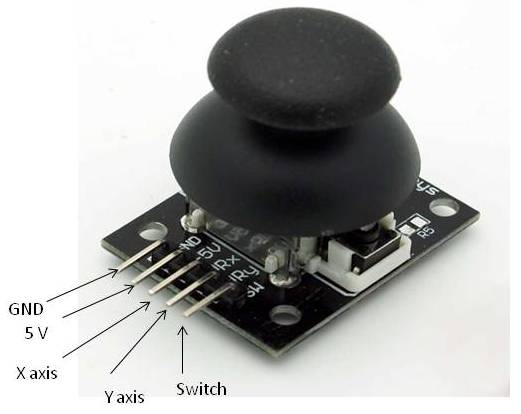
\includegraphics[scale=0.5]{joystick_pinout.jpg}
\caption{Joystick Pinout}
\end{figure}
\item
Now, use the inbuilt UART to communicate the digital values (i.e. both the X axis and the Y axis) to the computer. Use a terminal emulation software like Serial Terminal or Real Term to view the data being sent by the Tiva Board to your computer.
\newline
\hspace{10mm} \textit{The data sent should have the following syntax :}
\newline
\hspace{10mm}\textit{"X: Digital equivalent of the read value"}
\newline
\hspace{10mm}\textit{"Y: Digital equivalent of the read value"}
\item
Once you complete the above mentioned problem statements, you have to depict the values received in a graphical representation. In short, create a GUI which tracks the real time movements of the joystick.
\newline
Refer to the Figure 1, the circle marker should move to the left if the joystick button is tilted towards left and right if tilted towards right. The marker should remain at the centre when joystick is stationary.
\end{enumerate}
\begin{figure}
\centering
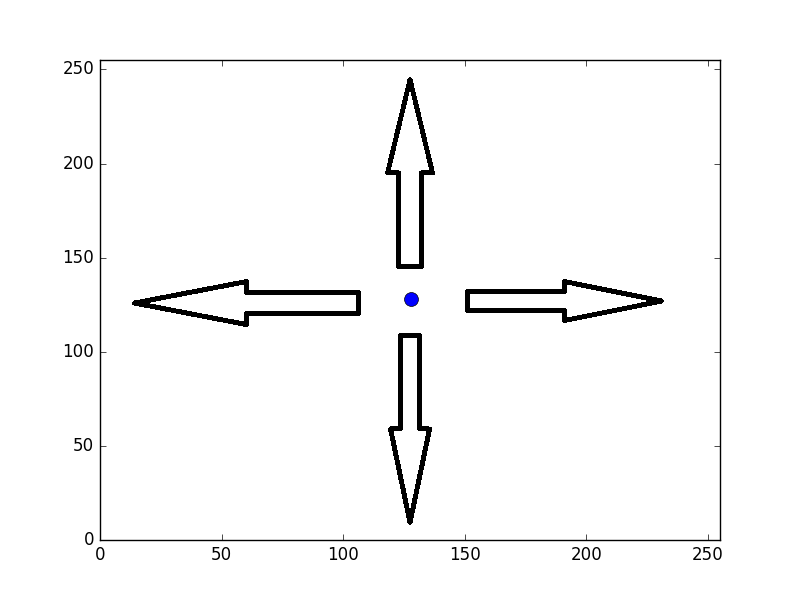
\includegraphics[scale=0.4]{joystickgui.jpg}
\caption{Joystick Graphical interface}
\end{figure}





%Relevant Theory
\section {Relevant Theory}
%%%%%%%%%%%%%%%%%%%%%%%
% FOR A NUMBERED LIST
% \begin{enumerate}
% \item Your_Item
% \end{enumerate}
%%%%%%%%%%%%%%%%%%%%%%%
Some general terms related to ADC.
\footnote{EE712 Embedded Systems, presentation from WEL Lab}
\begin{enumerate}
\item \textbf{Sample Sequencer}
The sampling control and data capture is handled by the sample sequencers.
The sample sequencers can be assumed to be a module with memory, which can sample different analog sources with a single trigger event without processor intervention.
All of the sequencers are identical in implementation except for the number of samples that can be captured and the depth of the FIFO.
\item \textbf{Trigger Source}
ADC can be triggered by various sources like processor, external GPIO, PWM, internal comparators, timer etc.
\item \textbf{Relative Priority}
There are 4 sample sequencers. Hence, we need to specify the relative priority of a sequencer in case we are using multiple sample sequencers.
\item \textbf{GPIO Pins}
There are 12 analog input channels shared by two Analog-to-Digital Converter modules. Certain GPIO pins can act as input channels for these ADC modules. For information about these pins, refer to section 12, pages 799 - 801 of this \href{http://www.ti.com/lit/ds/spms376e/spms376e.pdf}{\textbf{link}}. Use GPIOPinTypeADC() function to configure these pins.Refer to page 266 of this \href{http://www.ti.com/lit/ug/spmu298a/spmu298a.pdf}{\textbf{link}} detailed description of this function.
\end{enumerate}
Detailed description of theory and code examples are available in the following links:
\begin{enumerate}
\item Reference material 1: For ADC12 please go through \href{https://www.cse.iitb.ac.in/~erts/html_pages/Resources/Tiva/TM4C123G_LaunchPad_Workshop_Workbook.pdf}{\textbf{Resources7-Chapter 5}}.

\item Reference material 2:For UART please go through \href{https://www.cse.iitb.ac.in/~erts/html_pages/Resources/Tiva/TM4C123G_LaunchPad_Workshop_Workbook.pdf}{\textbf{Resources7-Chapter 12}}.
\end{enumerate}

\textbf{Joystick Graphical User Interface:}
\newline
You can use any open source programming language to build your GUI. Below, we have listed down some pointers to assist you, if you choose python
\begin{enumerate}
\item The first step is to read serial data coming on your COM port. Use pyserial library to do so.
\item If you notice carefully, GUI only requires five distinct values, you can avoid sending other values in your embedded C code. Also the rate at which Joystick data is sampled can also be reduced.
\item
Once you start receiving your required data, you can use matplotlib and drawnow library to get a real time Graphical representation. There are several other libraries that can be used to get a real time representation, you are free to use any of them. 
\end{enumerate}



%%%Procedure
%%%%%%%%%%%%%%%%%%%%%%%%%%%%%%
\section {Procedure}
\begin{enumerate}
\item For ADC and UART code :\\
	Include "adc.h" and "uart.h" header files.\\
    Enable ADC0 and ADC1 peripherals. Enable and configure the UART pins. Set the required Baud rate. \\
    Wait till ADC conversion is complete. Average the data obtained. This is then converted according to requirements. Send the ASCII value of this data to PC using UART.
\item To create GUI :\\
	Import serial library, matplotlib, numpy.\\
    Read the serial data.\\
    Enable the interactive plot using plt.ion() function.\\
    Split the received co-ordinates at comma and convert it into float.\\
    Plot these co-ordinates using "drawnow()" function.
    
\end{enumerate}


%%% Demo and Submissions
\section {Demo and Submissions}
%%%%%%%%%%%%%%%%%%%%%%%%%%%%%%%%%%%%%%%%%%%%%%%%
You have to shoot two individual videos demonstrating the output of the problem statement.
Your codes for each of the problem statement has to be uploaded in Github repository.
\end{document} % NOTHING AFTER THIS LINE IS PART OF THE DOCUMENT
